\documentclass[a4paper,fleqn]{cas-dc}
\usepackage[numbers]{natbib}
\usepackage{siunitx}
\usepackage{graphicx}
\usepackage{amsmath}

\shorttitle{When Does NMPC Outperform Robust PID?}
\shortauthors{G.M. de Andrade and E.R. Edwards}

% cas-dc places the keyword box in a zero-width hbox without \hss (spurious overfull warning)
\ExplSyntaxOn
\AddToHook{env/Abstract/begin}{\hbox_gset_to_wd:Nnn \g_stm_key_box {\c_zero_dim} {\box_use_drop:N \g_stm_key_box \hss}}
\ExplSyntaxOff

\begin{document}
\let\WriteBookmarks\relax
\def\floatpagepagefraction{1}
\def\textpagefraction{.001}

\title [mode = title]{When Does Nonlinear Model Predictive Control Outperform Robust PID? A Comparative Study under Fouling and Actuator Constraints}

\author[1]{Gabriel Marques de Andrade}
\cormark[1]
\ead{gmandrade.egm@uesc.br}
\credit{Conceptualization, Methodology, Software, Investigation, Writing -- original draft}

\author[1]{Elilton Rodrigues Edwards}
\ead{eredwards@uesc.br}
\credit{Supervision, Methodology, Writing -- review \& editing}

\affiliation[1]{organization={Department of Exact and Technological Sciences (DCET), State University of Santa Cruz (UESC)},
    addressline={Rodovia Jorge Amado, km 16},
    city={Ilh\'eus},
    postcode={45662-900},
    state={Bahia},
    country={Brazil}}

\cortext[1]{Corresponding author}

\begin{abstract}
When does the computational overhead of nonlinear model predictive control (NMPC) pay off in an exothermic reactor? This question is answered for a three-state continuous stirred tank reactor with jacket dynamics and a cooling valve limited in amplitude and slew rate. NMPC is compared only with robustly tuned PID baselines, AMIGO and an ITAE-optimal PID constrained to a maximum sensitivity of 1.6, all acting through the same valve with a rate-aware anti-windup. The NMPC uses a CasADi/IPOPT formulation with an RK4 prediction model and is evaluated with true-state access (Oracle) and with an augmented extended Kalman filter and moving-horizon estimator that reconstructs concentration and a fouling factor from two thermocouples. Near the design point the NMPC lowers the servo IAE of the best PID by only 2.3\%. After an abrupt loss of heat transfer to 70\% it reduces the IAE of the best PID by 21.0\%, and the output-feedback variant stays within 1.7\% of the Oracle. Without an integrating disturbance model, however, both NMPC variants keep an offset of about 9~K under unmeasured feed disturbances that both PID loops reject, and at 60\% heat transfer no controller reaches the setpoint within the run. Each NMPC sample costs 31--39~ms against 0.09~ms for PID. Five criteria summarize when nonlinear prediction is worth its cost.
\end{abstract}

\begin{highlights}
\item NMPC is benchmarked only against $M_s$-constrained PID on the same valve
\item Near the design point NMPC lowers the best PID servo IAE by only 2.3\%
\item After abrupt jacket fouling NMPC cuts the IAE of the best PID by 21.0\%
\item Without a disturbance model NMPC keeps an offset under unmeasured feed shocks
\end{highlights}


\begin{keywords}
Nonlinear model predictive control \sep Moving horizon estimation \sep Robust PID tuning \sep Exothermic CSTR \sep Heat-exchanger fouling \sep Actuator constraints
\end{keywords}

\maketitle

\section{Introduction}
\label{sec:introduction}
% ============================================================
%  Section 1: Introduction
% ============================================================

Nonlinear model predictive control (NMPC) is the natural candidate for exothermic reactors: it predicts with the Arrhenius kinetics instead of a local linearization, it handles valve amplitude and rate constraints explicitly, and modern tools such as CasADi/IPOPT and do-mpc solve the underlying optimal control problems in milliseconds \cite{rawlings2020model, hedengren2014nonlinear, fiedler2023dompc}. Fixed-gain PID control, by contrast, still regulates the large majority of industrial loops \cite{astrom2006pid, seborg2010process}. The engineering question is therefore not whether NMPC can beat PID, but \emph{when} the additional model, estimator and on-line optimization pay off over a PID loop that has been tuned as well as a practitioner can tune it.

Published comparisons rarely answer this question, for two reasons. First, the linear baseline is often a classical empirical tuning correlation derived for unconstrained linear plants and known to give small robustness margins \cite{odwyer2009handbook, garpinger2014performance}. Beating such a baseline shows that robustness matters, not that nonlinear prediction does. Robust rules that bound the maximum sensitivity $M_s$, such as AMIGO \cite{astrom2006pid}, SIMC \cite{skogestad2003simple, grimholt2018optimal} or direct optimization of a time-domain criterion under an $M_s$ constraint \cite{garpinger2014performance, padula2012optimal}, are the relevant references. Second, the PID loop is frequently simulated without the actuator the NMPC is constrained by, or with an anti-windup scheme that ignores the valve slew rate, so that integrator windup rather than the control law decides the comparison \cite{hippe2006windup, tarbouriech2009antiwindup, bohn1995analysis, peng1996nonlinear}. A fair benchmark gives both controllers the same saturating, rate-limited valve, the same measurements and the same evaluation protocol.

Exothermic continuous stirred tank reactors (CSTRs) are the canonical test bed for this comparison \cite{uppal1974dynamic, aris1958analysis, luyben2007chemical, bequette2003process}: the exponential temperature dependence of the reaction rate makes the process gain vary with the operating point, and jacket fouling reduces the heat-transfer capacity during operation. Nonlinear geometric and robust designs have been proposed for this class of process \cite{alvarez1995robust}, but their benefit over a robustly tuned PID acting through a rate-limited valve has not been quantified scenario by scenario.

This paper performs that quantification on a three-state CSTR with an explicit jacket energy balance and a cooling valve limited to $[0, 300]$~L/min and $80$~L/min$^2$. The NMPC is evaluated in two forms: with access to the true state (NMPC-Oracle), which bounds what nonlinear prediction can achieve, and with an augmented moving-horizon estimator that reconstructs the concentration and a fouling factor from two thermocouples (NMPC-MHE), which is the implementable controller. The linear baselines are the two best robust tunings of a broader benchmark of the same plant: AMIGO and a PID whose ITAE is minimized subject to $M_s \le 1.6$ on the identified dead-time model. Both PID loops use a directional anti-windup that freezes the integrator whenever the previous command was cut by the amplitude \emph{or} the slew-rate limit.

The contributions are:
\begin{enumerate}
    \item A controlled comparison of NMPC and robust PID on the same nonlinear plant, valve and measurements, over six scenarios: nominal servo step, unmeasured feed disturbances, abrupt and graded jacket fouling, wide-range multi-point tracking and Monte Carlo sensor noise.
    \item A formulation of output-feedback NMPC with an augmented state $[C_A, T, T_j, \alpha_{UA}]^\top$, estimated by an extended Kalman filter whose estimates serve as arrival-cost priors for a moving-horizon refinement, together with a study of its sensitivity to the estimator covariances and of its computational cost per sample.
    \item Five criteria, each supported by a specific scenario, that delimit when nonlinear control pays off on this reactor and when a robust PID is the better choice, including a structural explanation of the offset of NMPC under disturbances absent from its model.
\end{enumerate}
All tables and figures are generated by the released simulation scripts with fixed random seeds; no number in this paper is entered by hand.

The paper is organized as follows. Section~\ref{sec:formulation} presents the plant, the NMPC and the augmented estimator, Section~\ref{sec:baselines} the PID baselines, Section~\ref{sec:results} the results and Section~\ref{sec:conclusion} the conclusions.


\section{Plant model, NMPC and augmented moving-horizon estimator}
\label{sec:formulation}
% ============================================================
%  Section 2: Plant, NMPC and augmented MHE
% ============================================================

\subsection{Nonlinear CSTR with jacket dynamics and valve constraints}
\label{subsec:plant}
An irreversible exothermic reaction $A \rightarrow B$ takes place in a CSTR cooled by a jacket whose energy balance is modelled explicitly \cite{uppal1974dynamic, luyben2007chemical, seborg2010process}:
\begin{align}
    \frac{dC_A}{dt} &= \frac{q}{V}(C_{Af} - C_A) - r_A, \label{eq:cstr_ca} \\
    \frac{dT}{dt}   &= \frac{q}{V}(T_f - T) + \frac{(-\Delta H)}{\rho C_p} r_A - \frac{UA}{V \rho C_p}(T - T_j), \label{eq:cstr_t} \\
    \frac{dT_j}{dt} &= \frac{q_j}{V_j}(T_{jf} - T_j) + \frac{UA}{V_j \rho_j C_{pj}}(T - T_j), \label{eq:cstr_tj}
\end{align}
with $r_A = k_0 \exp(-E/RT)\,C_A$. The state is $\mathbf{x} = [C_A, T, T_j]^\top$, the manipulated input is the coolant flow $u = q_j$ and the controlled output is $T$. The parameters are $V = 100$~L, $V_j = 20$~L, $q = 100$~L/min, $C_{Af} = 1.0$~mol/L, $T_f = 350$~K, $T_{jf} = 300$~K, $k_0 = 7.2 \times 10^{10}$~min$^{-1}$, $E/R = 8750$~K, $-\Delta H = 5.0 \times 10^4$~cal/mol, $\rho C_p = \rho_j C_{pj} = 500$~cal/(L$\cdot$K) and $UA = 5.0 \times 10^4$~cal/(min$\cdot$K). At $\bar q_j = 100$~L/min the operating point is $\mathbf{x}_{ss} = [0.0502~\text{mol/L},\ 396.65~\text{K},\ 348.33~\text{K}]^\top$, a high-conversion steady state at which the Jacobian has three real negative eigenvalues.

The valve is bounded in amplitude and rate,
\begin{equation}
    0 \le q_j \le 300~\text{L/min}, \qquad \left|\frac{dq_j}{dt}\right| \le S_{\max} = 80~\text{L/min}^2,
    \label{eq:valve}
\end{equation}
so that a full stroke takes $3.75$~min. At the sampling interval $\Delta t = 0.02$~min the valve can move at most $S_{\max}\Delta t = 1.6$~L/min per sample. Jacket fouling is represented by a factor $\alpha_{UA} = UA_{\text{eff}}/UA_{\text{nom}}$ that multiplies $UA$ in Eqs.~\eqref{eq:cstr_t}--\eqref{eq:cstr_tj}. Both controller classes act through the same valve model and receive the same noisy thermocouple signals.

\subsection{Nonlinear model predictive control}
\label{subsec:nmpc}
The NMPC is implemented in \texttt{do-mpc} with CasADi and IPOPT \cite{fiedler2023dompc, rawlings2020model}. Its prediction model $\mathbf{F}$ is the zero-order-hold map of Eqs.~\eqref{eq:cstr_ca}--\eqref{eq:cstr_tj} over one sampling interval $\Delta t = 0.02$~min, computed with four fixed RK4 sub-steps per sample ($h = 0.005$~min), in which $UA$ is replaced by $\hat\alpha_{UA}\,UA_{\text{nom}}$ and the model is augmented with the previous valve position $u_{k-1}$. At every sample the controller solves
\begin{align}
    &\min_{u_0,\dots,u_{N-1}} \sum_{k=0}^{N} \left(T_k - T_{sp}\right)^2 + r\sum_{k=0}^{N-1}(u_k - u_{k-1})^2 \nonumber \\
    &\text{s.t.} \quad \mathbf{x}_{k+1} = \mathbf{F}(\mathbf{x}_k, u_k;\, \hat\alpha_{UA}), \nonumber \\
    &\phantom{\text{s.t.}} \quad 0 \le u_k \le 300, \quad |u_k - u_{k-1}| \le S_{\max}\,\Delta t,
    \label{eq:nmpc}
\end{align}
with $N = 50$ ($1.0$~min) and $r = 10^{-3}$; a horizon of $N = 75$ leaves the nominal IAE unchanged to four significant digits. The non-linear program (NLP) is solved at each sampling instant by IPOPT using the sparse linear solver MUMPS with an optimality tolerance $\epsilon_{\text{tol}} = 10^{-6}$ and a maximum iteration cap of $100$ iterations. The rate constraint is imposed on every predicted move, and the first move is projected onto the physical envelope before it is applied, so the NMPC cannot exploit a faster valve than the PID loops. The cost contains no integrating disturbance model; Section~\ref{subsec:load_results} shows the consequence.

Two feedback variants are compared:
\begin{itemize}
    \item \textbf{NMPC-Oracle} initializes Eq.~\eqref{eq:nmpc} with the true state $[C_A, T, T_j]$. Its fouling factor is tracked by the estimator described below, fed with noise-free thermocouples. It isolates the benefit of nonlinear prediction and constraint handling from estimation error and is not implementable, because $C_A$ is not measured on-line.
    \item \textbf{NMPC-MHE} reconstructs the state and the fouling factor from the noisy measurements $\mathbf{y}_k = [T_k,\ T_{j,k}]^\top$ only.
\end{itemize}

\subsection{Augmented extended Kalman filter and moving-horizon refinement}
\label{subsec:mhe}
The estimator works on the augmented state $\mathbf{x}_a = [C_A,\ T,\ T_j,\ \alpha_{UA}]^\top$, propagated with the plant equations and a random-walk model $\dot\alpha_{UA} = 0$. An extended Kalman filter (EKF) with the same RK4 map $\mathbf{F}$ performs
\begin{align}
    \hat{\mathbf{x}}_{k|k-1} &= \mathbf{F}(\hat{\mathbf{x}}_{k-1}, u_{k-1}), \nonumber \\
    P_{k|k-1} &= \Phi_k P_{k-1} \Phi_k^\top + Q_e, \quad \Phi_k = I + \Delta t\,\frac{\partial \mathbf{f}_a}{\partial \mathbf{x}_a}\Big|_{\hat{\mathbf{x}}_{k-1}}, \nonumber \\
    K_k &= P_{k|k-1} H^\top \left(H P_{k|k-1} H^\top + R_e\right)^{-1}, \nonumber \\
    \hat{\mathbf{x}}_k &= \hat{\mathbf{x}}_{k|k-1} + K_k\left(\mathbf{y}_k - H\hat{\mathbf{x}}_{k|k-1}\right), \label{eq:ekf}
\end{align}
where $H$ selects $(T, T_j)$ and
\begin{align}
    Q_e &= \mathrm{diag}(10^{-4}, 10^{-2}, 10^{-2}, 5\times10^{-4}), \nonumber \\
    R_e &= \mathrm{diag}(0.05, 0.05), \quad P_0 = \mathrm{diag}(0.05, 1.0, 1.0, 0.05). \nonumber
\end{align}
The EKF estimates at the start of a window of the last $N_m = 8$ samples serve as arrival-cost priors $(\hat C_A^{\text{prior}}, \hat\alpha_{UA}^{\text{prior}})$ for a moving-horizon refinement of the unmeasured pair \cite{rao2003constrained}:
\begin{multline}
    \min_{C_{A,0},\,\alpha_{UA}} \; 4\left\|\begin{bmatrix} C_{A,0} - \hat C_{A}^{\text{prior}} \\ \alpha_{UA} - \hat\alpha_{UA}^{\text{prior}}\end{bmatrix}\right\|^2 \\
    + \sum_{i=1}^{N_m - 1} \left[\left(T_i - \tilde T_i\right)^2 + \tfrac14\left(T_{j,i} - \tilde T_{j,i}\right)^2\right],
    \label{eq:mhe}
\end{multline}
subject to $0 \le C_{A,0} \le 1$ and $0.4 \le \alpha_{UA} \le 1.2$, where $(\tilde T_i, \tilde T_{j,i})$ result from chaining $\mathbf{F}$ forward from the window-start state $(C_{A,0}, T_0, T_{j,0}, \alpha_{UA})$ with the inputs actually applied. The moving-horizon non-linear program of Eq.~\eqref{eq:mhe} is solved at each sampling instant using a bounded trust-region reflective algorithm with convergence tolerance $10^{-6}$ and a cap of $50$ function evaluations. The optimal pair is propagated to the end of the window to give $\hat C_{A,k}$ and $\hat\alpha_{UA,k}$, which initialize Eq.~\eqref{eq:nmpc}. Because estimator and controller share the same RK4 model, the window residuals vanish on noise-free data, and NMPC-MHE then reproduces the Oracle trajectory exactly.

\paragraph{Tuning and observability.} The covariances follow physical scales rather than trial and error. $P_0$ assigns a standard deviation of $1$~K to the measured temperatures and about $0.22$ to $C_A$ and $\alpha_{UA}$, several times $C_{A,ss}$ and the full fouling range, so the unmeasured states start from an uninformative prior. $R_e = 0.05$~K$^2$ is deliberately larger than the thermocouple noise used in the benchmarks ($\sigma = 0.05$~K), which smooths the innovations. The random walk of $\alpha_{UA}$ ($5 \times 10^{-4}$ per sample) lets the estimate follow an abrupt loss of heat transfer within a few samples. The linearized augmented model at $\mathbf{x}_{ss}$ is locally observable: the matrix $[H;\, H\Phi;\, H\Phi^2;\, H\Phi^3]$ has full rank $4$ with both thermocouples and with $T$ alone, a property checked by the unit test suite. The moving-horizon step re-estimates $(C_{A,0}, \alpha_{UA})$ under bounds at every sample, which removes the dependence on the EKF linearization during fast transients. No formal convergence proof is claimed: the arrival cost is approximated by the EKF prior, and Section~\ref{subsec:mhe_tuning} tests the sensitivity to $R_e$ and $Q_\alpha$ empirically.


\section{Robust PID baselines}
\label{sec:baselines}
% ============================================================
%  Section 3: Robust PID baselines
% ============================================================

\subsection{Discrete PID with directional rate-aware clamping}
\label{subsec:pid}
Both baselines use the same discrete parallel PID with derivative on measurement \cite{astrom2006pid}, sampled at $\Delta t = 0.02$~min:
\begin{align}
    u_{\text{raw},k} &= \bar q_j + K_p e_k + I_k + D_k, \nonumber \\
    D_k &= \frac{\tau_f D_{k-1} - K_p T_d (y_k - y_{k-1})}{\tau_f + \Delta t}, \quad \tau_f = \frac{T_d}{10}, \label{eq:pid}
\end{align}
with $e_k = T_{sp,k} - y_k$, $y_k$ the measured temperature and $\bar q_j = 100$~L/min. Because the valve of Eq.~\eqref{eq:valve} is limited in amplitude \emph{and} rate, the applied input $u_{\text{act},k}$ differs from $u_{\text{raw},k}$ whenever either limit is active. The trapezoidal integrator is frozen when the previous command was cut and the current increment pushes in the same direction:
\begin{equation}
    I_k = \begin{cases}
        I_{k-1}, & \text{if } \left(u_{\text{raw},k-1} - u_{\text{act},k-1}\right)\delta I_k > 0, \\
        I_{k-1} + \delta I_k, & \text{otherwise,}
    \end{cases}
    \label{eq:clamping}
\end{equation}
with $\delta I_k = (K_p/T_i)\,\tfrac12(e_k + e_{k-1})\,\Delta t$. The product form handles the sign of the reverse-acting loop ($K_p < 0$) automatically, and including the slew-rate cut matters on this valve because a $2$~K setpoint step already demands more than $1.6$~L/min per sample from both tunings; an amplitude-only rule would keep integrating throughout the rate-limited ramp \cite{bohn1995analysis, peng1996nonlinear, hippe2006windup}. Evaluating the saturation residual at the previous sample avoids an algebraic loop between $I_k$ and the nonlinear valve map.

\subsection{Identified design model and tunings}
\label{subsec:tunings}
Both tunings use a first-order-plus-dead-time (FOPTD) model $G_p(s) = K e^{-\theta s}/(\tau s + 1)$ identified by least squares from an open-loop step $\Delta q_j = +10$~L/min at $\mathbf{x}_{ss}$; its parameters are listed in the caption of Table~\ref{tab:classical_benchmark}. The dead time is apparent: it lumps the lag of the jacket, and the loop is lag dominant ($\theta/\tau < 0.2$). Robustness is measured by the maximum sensitivity on this dead-time loop,
\begin{equation}
    M_s = \max_\omega \left|\frac{1}{1 + G_p(j\omega)C(j\omega)}\right|,
    \label{eq:ms}
\end{equation}
which is the relevant quantity for this loop: the delay-free Jacobian linearization has relative degree two and returns $M_s \approx 1$ for almost any gain, which would silently disable a robustness constraint.
\begin{itemize}
    \item \textbf{AMIGO} maximizes integral gain subject to a robustness constraint and is given in closed form for FOPTD processes \cite{astrom2006pid}:
    \begin{equation}
        \begin{gathered}
        K_p = \frac{1}{K}\left(0.2 + 0.45\frac{\tau}{\theta}\right), \\
        T_i = \frac{0.4\theta + 0.8\tau}{\theta + 0.1\tau}\,\theta, \quad T_d = \frac{0.5\theta\tau}{0.3\theta + \tau}.
        \end{gathered}
        \label{eq:amigo}
    \end{equation}
    \item \textbf{Optimal ITAE ($M_s \le 1.6$)} minimizes the closed-loop ITAE of the nominal servo step simulated on the nonlinear plant with the same valve,
    \begin{equation}
        \min_{K_p, T_i, T_d} \int_0^{t_{\text{sim}}} t\,|e(t)|\,dt \quad \text{s.t.} \quad M_s \le 1.6,
        \label{eq:opt}
    \end{equation}
    with $M_s$ from Eq.~\eqref{eq:ms} enforced by the quadratic penalty $10^4\max(0, M_s - 1.6)^2$. The Nelder--Mead search is started from a default guess and from every analytical tuning that already satisfies the constraint, and the best feasible optimum is kept, because the default start alone stops at a PI-like local optimum. The constraint is active at the optimum.
\end{itemize}
The resulting gains, and $M_s$, are listed in Table~\ref{tab:classical_benchmark}. Both PIDs are one-degree-of-freedom; setpoint weighting would change their servo response but not their disturbance rejection \cite{astrom2006pid}, which is where the comparison with NMPC is decided (Section~\ref{subsec:nmpc_results}).

These two tunings are the strongest linear competitors available for this loop: in a broader benchmark of the same plant and valve \cite{andrade2026robust}, Optimal ITAE gave the lowest nominal servo IAE of all PID tunings considered, and AMIGO the fastest recovery from the fouling event of Section~\ref{subsec:nmpc_results} among the robust PID loops.


\section{Results and discussion}
\label{sec:results}
% ============================================================
%  Section 4: Results and discussion
% ============================================================
% Every number quoted here is copied from the tables generated by
% experiments/build_paper_assets.py cace (CSV mirrors in results/cace/); none is typed by hand.

\subsection{Evaluation protocol}
\label{subsec:protocol}
All runs start at $\mathbf{x}_{ss}$ with $q_j = \bar q_j$ and use $\Delta t = 0.02$~min. The servo scenarios apply a $-2$~K setpoint step and last $10$~min. Error metrics are computed on the \emph{true} reactor temperature, $\mathrm{IAE} = \int_0^{t_f} |T_{sp} - T|\,dt$, so that sensor noise enters them only through its effect on the valve; ITAE weights the error by the time elapsed since the step. The total variation $\mathrm{TV} = |u_0 - \bar q_j| + \sum_k |u_k - u_{k-1}|$ measures valve travel and includes the first move. Because the valve moves at most $1.6$~L/min per sample, TV is bounded by $|u_0 - \bar q_j| + S_{\max} t_f \approx 800$~L/min over $10$~min. The four controllers are AMIGO, Optimal ITAE ($M_s \le 1.6$), NMPC-Oracle and NMPC-MHE (Sections~\ref{sec:formulation}--\ref{sec:baselines}). Noise is Gaussian with standard deviation $\sigma$ on the reactor thermocouple, and, for NMPC-MHE, on the jacket thermocouple as well; all random seeds are fixed.

\subsection{Nominal setpoint tracking}
\label{subsec:nominal}
Table~\ref{tab:classical_benchmark} and Fig.~\ref{fig:classical_benchmark} report the noise-free servo step. Both NMPC variants give identical trajectories ($\mathrm{IAE} = 0.808$~K$\cdot$min, $M_p = 5.2\%$, $\mathrm{TV} = 67.4$~L/min), because with a consistent RK4 model the estimator reconstructs $C_A$ exactly from $T$ and $T_j$. Optimal ITAE reaches $\mathrm{IAE} = 0.827$~K$\cdot$min with $M_p = 2.2\%$ and $t_s = 0.94$~min, and AMIGO $0.925$~K$\cdot$min with $M_p = 9.7\%$. Relative to Optimal ITAE the NMPC lowers the IAE by $2.3\%$ and the settling time from $0.94$ to $0.86$~min, while using $39\%$ more valve travel. Near the design point, where the identified FOPTD model is accurate, an $M_s$-constrained PID with correct anti-windup leaves little for nonlinear prediction to gain.

\begin{figure}[!t]
    \centering
    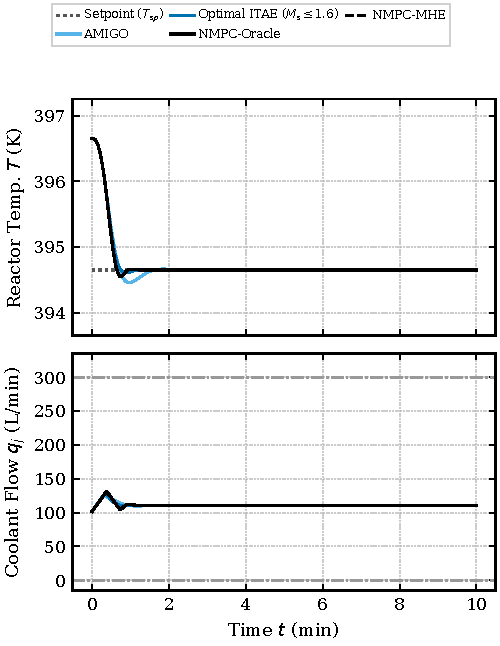
\includegraphics[width=\columnwidth]{figures/fig1_classical_benchmark.pdf}
    \caption{Nominal setpoint tracking ($-2$~K step at $t = 0$, noise-free): reactor temperature $T$ and coolant flow $q_j$ under the valve limits $[0, 300]$~L/min and $80$~L/min$^2$. NMPC-Oracle and NMPC-MHE coincide.}
    \label{fig:classical_benchmark}
\end{figure}

\begin{table*}[t]
\centering
\footnotesize
\caption{Nominal servo benchmark ($-2$~K setpoint step, noise-free) on the non-linear CSTR. FOPTD: $K=-0.1852$~K/(L/min), $\tau=0.6427$~min, $\theta=0.0935$~min. $M_s$ is evaluated on the dead-time FOPTD loop; TV includes the initial valve move from $\bar q_j$.}
\label{tab:classical_benchmark}
\resizebox{\ifdim\width>\textwidth\textwidth\else\width\fi}{!}{%
\begin{tabular}{lcccccccccc}
\toprule
Method & \(K_p\) & \(T_i\text{ (min)}\) & \(T_d\text{ (min)}\) & \(\beta\) & IAE & ITAE & TV (L/min) & \(M_p\text{ (\%)}\) & \(t_s\text{ (min)}\) & \(M_s\) \\
\midrule
AMIGO & -17.79 & 0.327 & 0.045 & 1.0 & 0.925 & 0.308 & 40.4 & 9.7 & 1.44 & 1.45 \\
Optimal ITAE ($M_s \leq 1.6$) & -23.55 & 0.465 & 0.032 & 1.0 & 0.827 & 0.204 & 48.6 & 2.2 & 0.94 & 1.60 \\
NMPC-Oracle & -- & -- & -- & -- & 0.808 & 0.190 & 67.4 & 5.2 & 0.86 & -- \\
NMPC-MHE & -- & -- & -- & -- & 0.808 & 0.190 & 67.4 & 5.2 & 0.86 & -- \\
\bottomrule
\end{tabular}%
}
\end{table*}


\subsection{Abrupt fouling event: where nonlinear control pays off}
\label{subsec:nmpc_results}
The decisive scenario combines a $-2$~K setpoint step at $t = 0.5$~min, an abrupt loss of heat transfer to $70\%\,UA$ at $t = 4$~min and thermocouple noise $\sigma = 0.05$~K (Table~\ref{tab:nmpc_oracle_benchmark}, Fig.~\ref{fig:nmpc_oracle}). The fouling event reduces the process gain from $q_j$ to $T$ and raises the coolant demand, so the controllers must move the valve to a new operating point while the reactor heats up.

\begin{figure}[!t]
    \centering
    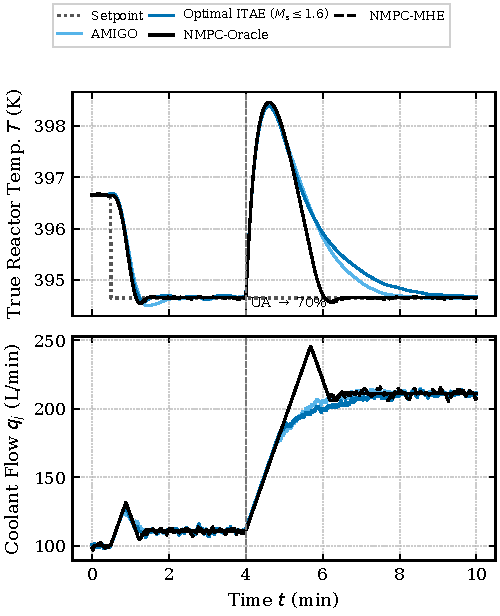
\includegraphics[width=\columnwidth]{figures/fig_nmpc_oracle_comparison.pdf}
    \caption{True reactor temperature and coolant flow under a $-2$~K step at $t = 0.5$~min, abrupt fouling to $70\%\,UA$ at $t = 4$~min (dashed line) and sensor noise $\sigma = 0.05$~K.}
    \label{fig:nmpc_oracle}
\end{figure}

\begin{table*}[t]
\centering
\footnotesize
\caption{Output-feedback gap: NMPC with true-state access (Oracle) vs NMPC with augmented MHE (thermal measurements only) vs $M_s$-constrained PID. $-2$~K step at $t=0.5$~min, jacket fouling to $70\%\,UA$ at $t=4$~min, sensor noise $\sigma=0.05$~K. Both NMPCs: $N=50$ ($1.0$~min), $|\Delta q_j| \le 80\,\Delta t$. Step time is the mean wall-clock time per sample (controller + plant integration; hardware dependent).}
\label{tab:nmpc_oracle_benchmark}
\resizebox{\ifdim\width>\textwidth\textwidth\else\width\fi}{!}{%
\begin{tabular}{lccccccc}
\toprule
Controller & IAE & \(\Delta\)IAE vs Oracle (\%) & ITAE & TV (L/min) & \(M_p\) (\%) & \(\hat\alpha_{UA}(t_f)\) & Step time (ms) \\
\midrule
AMIGO & 6.932 & +26.6 & 31.412 & 672.1 & 7.6 & -- & 0.09 \\
Optimal ITAE ($M_s \leq 1.6$) & 7.320 & +33.7 & 34.853 & 694.4 & 3.3 & -- & 0.09 \\
NMPC-Oracle & 5.474 & +0.0 & 23.034 & 252.4 & 5.2 & 0.700 & 31.46 \\
NMPC-MHE & 5.568 & +1.7 & 23.495 & 571.0 & 5.8 & 0.699 & 39.28 \\
\bottomrule
\end{tabular}%
}
\end{table*}


Among the PID loops, AMIGO recovers faster from the loss of cooling ($\mathrm{IAE} = 6.932$~K$\cdot$min) than Optimal ITAE ($7.320$~K$\cdot$min), because it has the larger integral gain ($|K_p|/T_i = 54.4$ versus $50.6$~min$^{-1}$, Table~\ref{tab:classical_benchmark}), at the price of a larger overshoot ($7.6\%$ versus $3.3\%$). The ranking of the nominal step is thus reversed: the tuning that is best for servo tracking is not the best after a change of the plant. NMPC-Oracle reaches $\mathrm{IAE} = 5.474$~K$\cdot$min, i.e. $21.0\%$ below AMIGO and $25.2\%$ below Optimal ITAE, with less than half of their valve travel ($252.4$ versus $672.1$ and $694.4$~L/min). After the event the estimator identifies the loss of heat transfer, and the NMPC re-plans the coolant trajectory to the new operating point against the rate limit; at $t_f$ the estimate is $\hat\alpha_{UA} = 0.700$ (Oracle) and $0.699$ (MHE) for a true value of $0.70$.

The output-feedback variant stays within $1.7\%$ of the Oracle in IAE ($5.568$~K$\cdot$min), so the two thermal measurements carry enough information to reconstruct both $C_A$ and $\alpha_{UA}$. The price of output feedback appears in the valve travel ($571.0$ versus $252.4$~L/min), which is still below that of both PID loops: the estimator propagates part of the measurement noise into the optimizer's initial state.

\paragraph{Computational cost.} The last column of Table~\ref{tab:nmpc_oracle_benchmark} gives the mean wall-clock time per sample, including the plant integration, measured on a desktop CPU: $31.46$~ms for NMPC-Oracle, $39.28$~ms for NMPC-MHE and $0.09$~ms for each PID loop. The moving-horizon estimator adds about $8$~ms per sample to the NMPC. Both NMPCs are thus several hundred times more expensive than a PID loop, but use less than $4\%$ of the $1.2$~s sampling interval, so real-time feasibility is not the limiting factor on this process. These times are hardware dependent; their ratio, not their absolute value, is the transferable result.

\subsection{Sensitivity of NMPC-MHE to the estimator covariances}
\label{subsec:mhe_tuning}
Table~\ref{tab:mhe_tuning} repeats the NMPC-MHE run of Table~\ref{tab:nmpc_oracle_benchmark} with the measurement covariance $R_e$ and the fouling random-walk variance $Q_\alpha$ scaled by $0.1$ and $10$. The nominal row reproduces Table~\ref{tab:nmpc_oracle_benchmark} ($\mathrm{IAE} = 5.568$~K$\cdot$min, $\mathrm{TV} = 571.0$~L/min).

\begin{table*}[t]
\centering
\footnotesize
\caption{Sensitivity of NMPC-MHE to the estimator covariances on the scenario of Table~\ref{tab:nmpc_oracle_benchmark} (fouling to $70\%\,UA$ at $t = 4$~min, $\sigma = 0.05$~K). $R_e$ is scaled as a whole, $Q_{\alpha}$ is the fouling random-walk variance. Settling: time after the fouling event from which $|\hat\alpha_{UA} - \alpha_{UA}| \le 0.02$ holds until $t_f$.}
\label{tab:mhe_tuning}
\resizebox{\ifdim\width>\textwidth\textwidth\else\width\fi}{!}{%
\begin{tabular}{lccccc}
\toprule
Covariance scaling & IAE & TV (L/min) & RMS \(\hat C_A - C_A\) (mol/L) & \(\hat\alpha_{UA}(t_f)\) & \(\alpha\) settling (min) \\
\midrule
Nominal & 5.568 & 571.0 & 6.97e-05 & 0.699 & 0.14 \\
\(R_e \times 0.1\) & 5.558 & 590.8 & 7.41e-05 & 0.699 & 0.14 \\
\(R_e \times 10\) & 5.574 & 508.8 & 6.18e-05 & 0.699 & 0.14 \\
\(Q_{\alpha} \times 0.1\) & 5.569 & 570.6 & 6.97e-05 & 0.699 & 0.14 \\
\(Q_{\alpha} \times 10\) & 5.567 & 571.7 & 6.97e-05 & 0.699 & 0.14 \\
\bottomrule
\end{tabular}%
}
\end{table*}


Over two decades of each covariance the fouling estimate enters the $\pm 0.02$ band within $0.14$~min of the event and ends at $\hat\alpha_{UA} = 0.699$, the RMS error of $\hat C_A$ stays between $6.18 \times 10^{-5}$ and $7.41 \times 10^{-5}$~mol/L, and the IAE varies only between $5.558$ and $5.574$~K$\cdot$min. $Q_\alpha$ has practically no effect, because the fouling factor is re-estimated at every sample by the moving-horizon refinement rather than propagated by the EKF. $R_e$ acts as a smoothing knob that trades valve travel ($590.8$~L/min for $R_e \times 0.1$, $508.8$~L/min for $R_e \times 10$) against a marginal change in tracking error. On this observable process the estimator does not require fine covariance tuning.

\subsection{Graded fouling and the thermodynamic boundary}
\label{subsec:fouling_results}
Table~\ref{tab:fouling_sensitivity} and Fig.~\ref{fig:fouling_robustness} report a deterministic sweep $UA \in \{100, 90, 80, 70, 60\}\%$ of the nominal value. Every run starts from the clean-jacket steady state, and the reduced $UA$ acts from $t = 0$ together with the setpoint step; the controllers must therefore reject the loss of cooling and track the new setpoint simultaneously. The $100\%$ rows reproduce Table~\ref{tab:classical_benchmark}.

\begin{figure*}[!t]
    \centering
    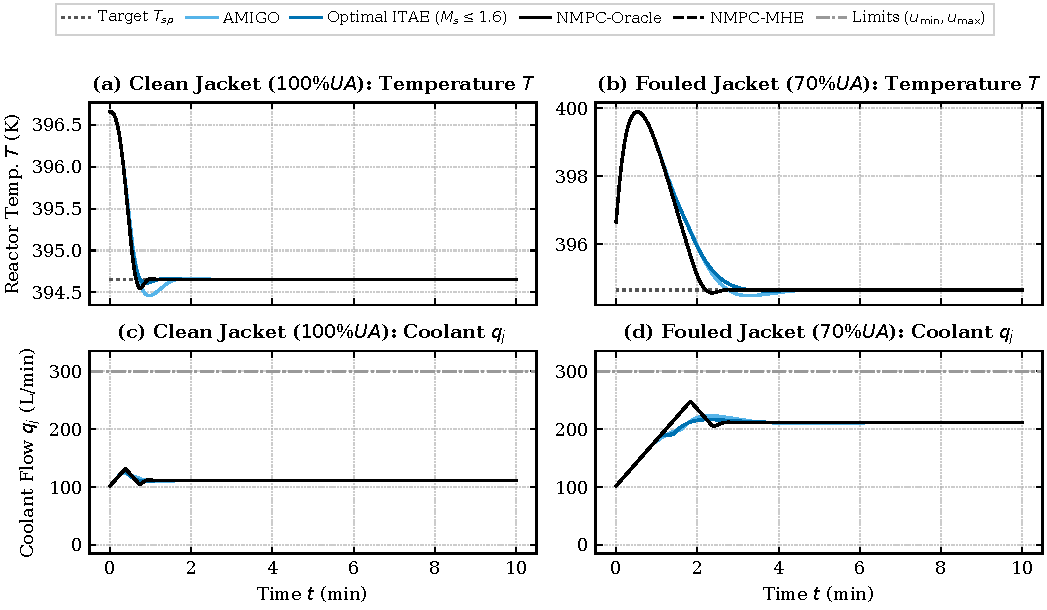
\includegraphics[width=0.98\textwidth]{figures/fig3_fouling_robustness.pdf}
    \caption{Effect of heat-transfer degradation (deterministic, start from the clean-jacket steady state): clean jacket ($100\%\,UA$) versus fouled jacket ($70\%\,UA$).}
    \label{fig:fouling_robustness}
\end{figure*}

\begin{table*}[t]
\centering
\footnotesize
\caption{Impact of heat exchanger fouling ($UA$ reduction from $100\%$ to $60\%$) on closed-loop tracking metrics.}
\label{tab:fouling_sensitivity}
\resizebox{\ifdim\width>\textwidth\textwidth\else\width\fi}{!}{%
\begin{tabular}{lccccc}
\toprule
Method & $UA / UA_{\text{nom}}$ & IAE & ITAE & TV (L/min) & $M_p$ (\%) \\
\midrule
AMIGO & 100\% & 0.93 & 0.31 & 40.4 & 9.7 \\
AMIGO & 90\% & 1.75 & 0.78 & 54.4 & 9.7 \\
AMIGO & 80\% & 3.56 & 2.27 & 90.0 & 11.2 \\
AMIGO & 70\% & 7.83 & 7.73 & 147.8 & 8.5 \\
AMIGO & 60\% & 31.08 & 115.44 & 209.1 & 0.0 \\
Optimal ITAE ($M_s \leq 1.6$) & 100\% & 0.83 & 0.20 & 48.6 & 2.2 \\
Optimal ITAE ($M_s \leq 1.6$) & 90\% & 1.72 & 0.71 & 56.8 & 0.0 \\
Optimal ITAE ($M_s \leq 1.6$) & 80\% & 3.48 & 2.06 & 73.1 & 0.1 \\
Optimal ITAE ($M_s \leq 1.6$) & 70\% & 7.76 & 7.44 & 143.0 & 1.4 \\
Optimal ITAE ($M_s \leq 1.6$) & 60\% & 30.79 & 114.60 & 205.8 & 0.0 \\
NMPC-Oracle & 100\% & 0.81 & 0.19 & 67.4 & 5.2 \\
NMPC-Oracle & 90\% & 1.57 & 0.55 & 92.0 & 5.5 \\
NMPC-Oracle & 80\% & 3.19 & 1.67 & 129.5 & 5.7 \\
NMPC-Oracle & 70\% & 6.95 & 5.70 & 196.7 & 4.3 \\
NMPC-Oracle & 60\% & 30.56 & 113.90 & 200.0 & 0.0 \\
NMPC-MHE & 100\% & 0.81 & 0.19 & 67.4 & 5.2 \\
NMPC-MHE & 90\% & 1.57 & 0.55 & 92.0 & 5.5 \\
NMPC-MHE & 80\% & 3.19 & 1.67 & 129.5 & 5.7 \\
NMPC-MHE & 70\% & 6.95 & 5.70 & 196.7 & 4.3 \\
NMPC-MHE & 60\% & 30.56 & 113.90 & 200.0 & 0.0 \\
\bottomrule
\end{tabular}%
}
\end{table*}


The NMPC advantage grows with the mismatch between the plant and the conditions the PID loops were tuned for: at $70\%\,UA$ both NMPC variants give $\mathrm{IAE} = 6.95$~K$\cdot$min against $7.76$ (Optimal ITAE) and $7.83$~K$\cdot$min (AMIGO), $10.4\%$ below the better PID. The gain is smaller than in the fouling event of Section~\ref{subsec:nmpc_results}; a plausible reason is that here the loss of cooling coincides with the setpoint step, so all controllers start the same large valve move at $t = 0$, whereas in the event the PID loops are surprised by the loss of cooling after having settled with a clean jacket. At $60\%\,UA$ the advantage vanishes: all four controllers give $\mathrm{IAE} = 30.56$--$31.08$~K$\cdot$min, and $M_p = 0.0\%$ because the temperature stays above the setpoint during the whole run. The NMPC travel of exactly $200.0$~L/min corresponds to a single monotone ramp from $100$ to the $300$~L/min limit, and the PID loops also end the run with the valve fully open. With the valve fully open, the heat-removal capacity of the jacket does not let the reactor reach the setpoint within $10$~min, and no control law acting through the same valve can change this.

\subsection{Unmeasured feed disturbances: the offset of NMPC}
\label{subsec:load_results}
Two sequential unmeasured shocks were applied at constant setpoint with $\sigma = 0.05$~K: a feed temperature step $\Delta T_f = +5$~K at $t = 2$~min and a feed concentration step $\Delta C_{Af} = +0.2$~mol/L ($+20\%$) at $t = 8$~min (Table~\ref{tab:load_disturbance}, Fig.~\ref{fig:disturbance_rejection}).

\begin{figure}[!t]
    \centering
    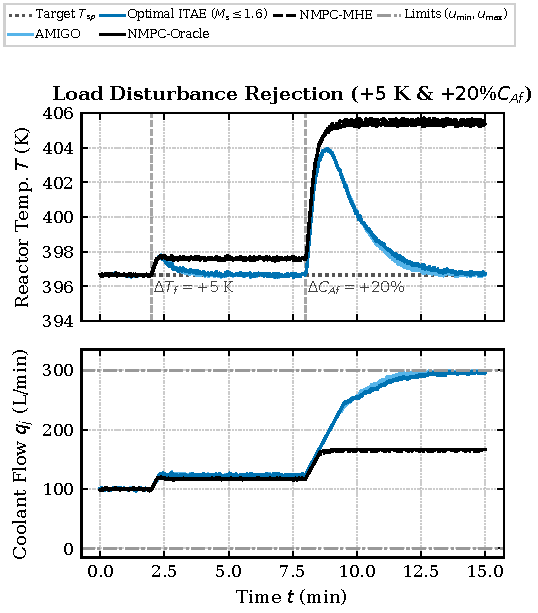
\includegraphics[width=\columnwidth]{figures/fig2_disturbance_rejection.pdf}
    \caption{Unmeasured load disturbances: $+5$~K feed temperature step at $t = 2$~min followed by a $+20\%$ feed concentration step at $t = 8$~min (sensor noise $\sigma = 0.05$~K).}
    \label{fig:disturbance_rejection}
\end{figure}

\begin{table*}[t]
\centering
\footnotesize
\caption{Regulatory performance under combined feed temperature ($+5$~K) and concentration ($+20\%$) load disturbances. $T(t_f) - T_{sp}$ is the true temperature error at $t_f = 15$~min; $\hat\alpha_{UA}(t_f)$ is the NMPC fouling estimate (true value $1.0$, no fouling in this test).}
\label{tab:load_disturbance}
\resizebox{\ifdim\width>\textwidth\textwidth\else\width\fi}{!}{%
\begin{tabular}{lccccccc}
\toprule
Method & IAE & ITAE & TV (L/min) & Peak Dev (K) & Max Valve (L/min) & \(T(t_f) - T_{sp}\) (K) & \(\hat\alpha_{UA}(t_f)\) \\
\midrule
AMIGO & 15.27 & 139.03 & 1013.8 & 7.29 & 299.5 & +0.02 & -- \\
Optimal ITAE ($M_s \leq 1.6$) & 16.20 & 150.00 & 1036.5 & 7.28 & 298.8 & +0.07 & -- \\
NMPC-Oracle & 63.91 & 706.75 & 75.9 & 8.82 & 166.6 & +8.69 & 0.981 \\
NMPC-MHE & 65.17 & 722.28 & 511.8 & 9.04 & 165.6 & +8.91 & 0.985 \\
\bottomrule
\end{tabular}%
}
\end{table*}


Both PID loops return to the setpoint ($T(t_f) - T_{sp} = +0.02$~K for AMIGO and $+0.07$~K for Optimal ITAE) with $\mathrm{IAE} = 15.27$ and $16.20$~K$\cdot$min, driving the valve close to its limit ($299.5$ and $298.8$~L/min). The NMPC variants perform worst ($\mathrm{IAE} = 63.91$ and $65.17$~K$\cdot$min, peak deviation $8.82$ and $9.04$~K) and do not return to the setpoint: at $t_f = 15$~min the error is $+8.69$~K (Oracle) and $+8.91$~K (MHE), with the valve stopped near $166$~L/min (maximum $166.6$ and $165.6$~L/min). The mechanism is structural:
\begin{enumerate}
    \item \textbf{No integral action.} The cost of Eq.~\eqref{eq:nmpc} penalizes the predicted error of a model that still assumes the nominal $T_f$ and $C_{Af}$. Re-initializing the prediction from the measured or true state at every sample is state feedback, not integral action: once the plant settles, the optimizer finds that the nominal model already reaches $T_{sp}$ with the current input and stops moving the valve. The residual error reflects the heat-load mismatch between the real feed and the model, which is why even the Oracle, with perfect state knowledge, keeps an $8.69$~K offset.
    \item \textbf{The estimator absorbs the wrong disturbance.} The only adapted quantity, $\hat\alpha_{UA}$, was introduced for fouling. Under the feed shocks it drifts to $0.981$ (Oracle) and $0.985$ (MHE) although no fouling occurs: the estimator explains part of the extra heat release as a loss of heat transfer. This partial compensation is far too small to remove the offset, and in operation it would raise a false fouling alarm.
    \item \textbf{What is missing.} Offset-free MPC augments the prediction model with integrating disturbance states, estimates them with the plant states and recomputes the steady-state target at every sample \cite{muske2002disturbance, pannocchia2003disturbance, rawlings2020model}. Zero offset requires the augmented model to be detectable, which limits the number of integrating disturbances to the number of measured outputs, here two. With $\alpha_{UA}$ occupying one of these slots, a fouling-plus-feed design must choose which disturbances to model or add a measurement, such as the outlet concentration.
\end{enumerate}
These limitations apply to any model-based controller whose model omits the disturbance that actually occurs, not only to the NMPC implemented here.

\subsection{Robustness to sensor noise}
\label{subsec:noise_results}
Table~\ref{tab:noise_sensitivity} and Fig.~\ref{fig:noise_sensitivity} report a Monte Carlo campaign with $30$ noise realizations per level, $\sigma \in \{0.0, 0.1, 0.2, 0.5, 1.0\}$~K, on the nominal servo step ($600$ closed-loop simulations).

\begin{figure}[!t]
    \centering
    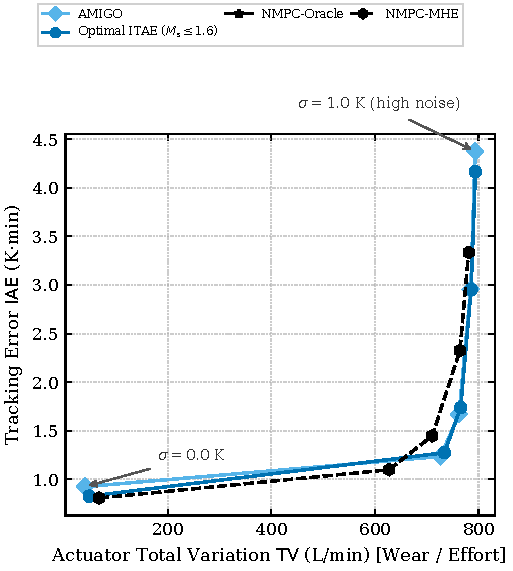
\includegraphics[width=\columnwidth]{figures/fig_noise_sensitivity.pdf}
    \caption{Mean true-temperature tracking error versus mean valve travel as the sensor noise grows from $\sigma = 0$ to $1.0$~K ($30$ Monte Carlo runs per point).}
    \label{fig:noise_sensitivity}
\end{figure}

\begin{table*}[t]
\centering
\footnotesize
\caption{Sensitivity of tracking error (IAE) and actuator effort (TV) to measurement noise levels across $30$ Monte Carlo runs.}
\label{tab:noise_sensitivity}
\resizebox{\ifdim\width>\textwidth\textwidth\else\width\fi}{!}{%
\begin{tabular}{lccc}
\toprule
Method & Noise $\sigma$ (K) & IAE (mean $\pm$ std) & TV (L/min) \\
\midrule
AMIGO & 0.0 & 0.93 $\pm$ 0.00 & 40.4 $\pm$ 0.0 \\
AMIGO & 0.1 & 1.24 $\pm$ 0.05 & 727.0 $\pm$ 7.7 \\
AMIGO & 0.2 & 1.67 $\pm$ 0.14 & 762.2 $\pm$ 6.5 \\
AMIGO & 0.5 & 2.96 $\pm$ 0.46 & 785.0 $\pm$ 5.0 \\
AMIGO & 1.0 & 4.38 $\pm$ 0.92 & 793.5 $\pm$ 1.9 \\
Optimal ITAE ($M_s \leq 1.6$) & 0.0 & 0.83 $\pm$ 0.00 & 48.6 $\pm$ 0.0 \\
Optimal ITAE ($M_s \leq 1.6$) & 0.1 & 1.27 $\pm$ 0.05 & 734.1 $\pm$ 6.8 \\
Optimal ITAE ($M_s \leq 1.6$) & 0.2 & 1.74 $\pm$ 0.12 & 765.5 $\pm$ 6.4 \\
Optimal ITAE ($M_s \leq 1.6$) & 0.5 & 2.95 $\pm$ 0.48 & 785.7 $\pm$ 3.0 \\
Optimal ITAE ($M_s \leq 1.6$) & 1.0 & 4.16 $\pm$ 0.63 & 794.0 $\pm$ 3.3 \\
NMPC-Oracle & 0.0 & 0.81 $\pm$ 0.00 & 67.4 $\pm$ 0.0 \\
NMPC-Oracle & 0.1 & 0.81 $\pm$ 0.00 & 67.4 $\pm$ 0.0 \\
NMPC-Oracle & 0.2 & 0.81 $\pm$ 0.00 & 67.4 $\pm$ 0.0 \\
NMPC-Oracle & 0.5 & 0.81 $\pm$ 0.00 & 67.4 $\pm$ 0.0 \\
NMPC-Oracle & 1.0 & 0.81 $\pm$ 0.00 & 67.4 $\pm$ 0.0 \\
NMPC-MHE & 0.0 & 0.81 $\pm$ 0.00 & 67.4 $\pm$ 0.0 \\
NMPC-MHE & 0.1 & 1.10 $\pm$ 0.04 & 627.6 $\pm$ 10.5 \\
NMPC-MHE & 0.2 & 1.45 $\pm$ 0.09 & 710.7 $\pm$ 9.0 \\
NMPC-MHE & 0.5 & 2.33 $\pm$ 0.22 & 764.2 $\pm$ 6.1 \\
NMPC-MHE & 1.0 & 3.33 $\pm$ 0.26 & 780.9 $\pm$ 5.9 \\
\bottomrule
\end{tabular}%
}
\end{table*}


\begin{enumerate}
    \item \textbf{NMPC-Oracle is invariant to sensor noise} ($\mathrm{IAE} = 0.81 \pm 0.00$~K$\cdot$min, $\mathrm{TV} = 67.4 \pm 0.0$~L/min at every $\sigma$): it reads the true state and feeds its fouling estimator noise-free thermocouples. It shows what an ideal sensor would allow, not what an implementable controller achieves.
    \item \textbf{Output feedback removes the noise immunity of NMPC in valve travel.} At $\sigma = 0.1$~K NMPC-MHE needs $627.6$~L/min against $727.0$ (AMIGO) and $734.1$~L/min (Optimal ITAE); at $\sigma \ge 0.5$~K all three approach the slew-rate ceiling of about $800$~L/min ($764.2$--$794.0$~L/min).
    \item \textbf{NMPC-MHE converts less noise into thermal deviation.} Its IAE grows from $0.81$ to $3.33 \pm 0.26$~K$\cdot$min at $\sigma = 1.0$~K, against $4.16 \pm 0.63$ (Optimal ITAE) and $4.38 \pm 0.92$~K$\cdot$min (AMIGO). The estimator filters the measurement through a physical model, whereas the PID loops act on the raw signal; the derivative filter ($N = 10$) bounds their high-frequency gain at $|K_p|(1 + N)$, which with $|K_p| = 17.79$--$23.55$ still maps $0.1$~K of noise into several L/min per sample.
\end{enumerate}

\subsection{Wide-range multi-point tracking}
\label{subsec:multistep}
A setpoint sequence $396.65 \rightarrow 390.0 \rightarrow 402.0 \rightarrow 396.65$~K over $24$~min with $\sigma = 0.05$~K moves the reactor across operating points with different Arrhenius gains (Table~\ref{tab:multistep_tracking}, Fig.~\ref{fig:multistep_tracking}).

\begin{figure}[!t]
    \centering
    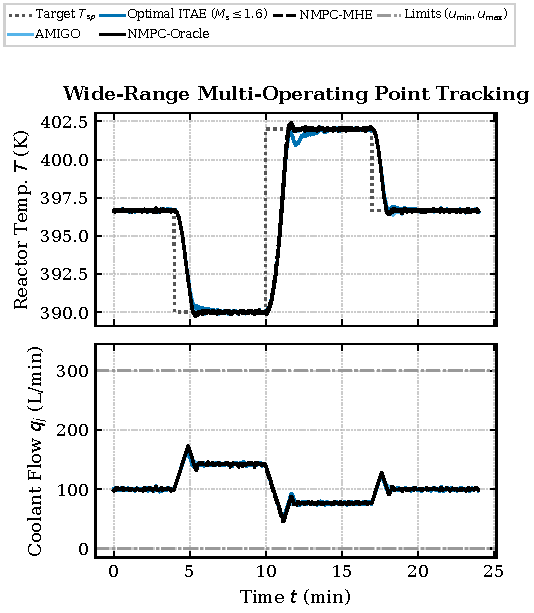
\includegraphics[width=\columnwidth]{figures/fig5_multistep_tracking.pdf}
    \caption{Wide-range setpoint tracking across the moderate ($390.0$~K), nominal ($396.65$~K) and strongly exothermic ($402.0$~K) operating points ($\sigma = 0.05$~K).}
    \label{fig:multistep_tracking}
\end{figure}

\begin{table*}[t]
\centering
\footnotesize
\caption{Multi-operating point tracking across moderate (390~K), nominal (396.65~K), and highly exothermic (402~K) reaction regimes.}
\label{tab:multistep_tracking}
\resizebox{\ifdim\width>\textwidth\textwidth\else\width\fi}{!}{%
\begin{tabular}{lccccc}
\toprule
Method & Total IAE & Total ITAE & Total TV (L/min) & Max Valve (L/min) & Min Valve (L/min) \\
\midrule
AMIGO & 20.50 & 208.02 & 1596.7 & 158.4 & 52.7 \\
Optimal ITAE ($M_s \leq 1.6$) & 21.43 & 218.85 & 1650.2 & 166.0 & 48.3 \\
NMPC-Oracle & 19.98 & 201.91 & 388.7 & 173.2 & 46.3 \\
NMPC-MHE & 19.66 & 198.36 & 1221.0 & 173.0 & 45.9 \\
\bottomrule
\end{tabular}%
}
\end{table*}


All controllers remain stable and below saturation (valve range $45.9$--$173.2$~L/min). The error differences are small: AMIGO $20.50$, Optimal ITAE $21.43$, NMPC-Oracle $19.98$ and NMPC-MHE $19.66$~K$\cdot$min, so the Oracle is $2.5\%$ below AMIGO. The decisive difference is valve activity: NMPC-Oracle needs $388.7$~L/min of travel against $1596.7$ (AMIGO) and $1650.2$~L/min (Optimal ITAE), about four times less, because it plans each transition against the slew-rate limit instead of reacting to the error. NMPC-MHE, which sees the same noise as the PID loops, needs $1221.0$~L/min, $24\%$ less than AMIGO.

\subsection{When and why nonlinear control outperforms robust PID}
\label{subsec:when_why}
The six scenarios separate the effect of the model from that of the information available to the controller. Nonlinear prediction pays off when the plant leaves the neighbourhood in which the PID was tuned and the change is represented in the model: after the fouling event, a fixed linear controller is tuned for one process gain, and Bode's sensitivity integral \cite{stein2003respect} forces any reduction of $|S(j\omega)|$ at low frequency to be paid by amplification elsewhere, so a single gain cannot be both fast and robust across the gain variation induced by fouling and by the Arrhenius term. The NMPC avoids this trade-off by re-linearizing implicitly at every sample, by updating $\hat\alpha_{UA}$ and by planning the valve ramp against the rate limit. Where the plant stays near the design point, or the disturbance is not represented in the model, the PID loops are equal or better, and integral action, not prediction, is what decides regulation. Neither class of controller crosses the boundary set by the heat-removal capacity of the jacket. Section~\ref{sec:conclusion} condenses these observations into five criteria.

\paragraph{Limitations.} The study uses one reactor, one valve and one fouling magnitude for the estimator study; the plant and the NMPC share the same model structure, so the results bound the benefit of NMPC under structural model match and parametric (fouling) mismatch only. The step times were measured on a single desktop computer. Offset-free NMPC and the PID loops with setpoint weighting were not part of this comparison.


\section{Conclusions}
\label{sec:conclusion}
% ============================================================
%  Section 5: Conclusions
% ============================================================

This paper compared a slew-rate-constrained NMPC, with true-state access (Oracle) and with an augmented EKF/moving-horizon estimator (NMPC-MHE), against the two strongest robust PID tunings of an exothermic CSTR, AMIGO and Optimal ITAE with $M_s \le 1.6$, all acting through the same saturating, rate-limited valve with directional anti-windup on the PID side. Five criteria delimit when the computational overhead of nonlinear control pays off on this reactor:
\begin{enumerate}
    \item \textbf{Near the design point, an $M_s$-constrained PID is sufficient.} The NMPC improves the nominal servo IAE of Optimal ITAE by $2.3\%$ and the wide-range tracking IAE of AMIGO by $2.5\%$. The relevant baseline for a nonlinear controller is a robustly tuned PID with correct anti-windup.
    \item \textbf{Nonlinear prediction pays off after a change of the plant that the model represents.} After an abrupt loss of heat transfer to $70\%\,UA$, NMPC-Oracle reduces the IAE of the best PID (AMIGO) by $21.0\%$ and that of Optimal ITAE by $25.2\%$, with less than half of their valve travel; NMPC-MHE stays within $1.7\%$ of the Oracle. In wide-range tracking the Oracle needs about four times less valve travel than the PID loops.
    \item \textbf{Without a disturbance model, nonlinear prediction does not help regulation.} Under unmeasured feed shocks both NMPC variants settle with an offset of $+8.69$ and $+8.91$~K, while both PID loops return to the setpoint. Offset-free formulations with integrating disturbance states are a prerequisite for using NMPC as a regulator on this process.
    \item \textbf{Output feedback removes part of the advantage.} The Oracle is invariant to sensor noise; NMPC-MHE, the implementable variant, uses valve travel comparable to that of a PID loop once $\sigma \ge 0.1$~K, although it still converts less noise into thermal deviation ($\mathrm{IAE} = 3.33$ versus $4.16$~K$\cdot$min at $\sigma = 1.0$~K).
    \item \textbf{No controller crosses the thermodynamic boundary.} At $60\%\,UA$ all four controllers give practically the same error ($30.56$--$31.08$~K$\cdot$min) with the valve driven to its limit; the boundary is set by the heat-removal capacity of the jacket, not by the control law.
\end{enumerate}
The cost of these benefits is moderate: $31.46$ and $39.28$~ms per sample for NMPC-Oracle and NMPC-MHE against $0.09$~ms for a PID loop, well within the $1.2$~s sampling interval. The practical recommendation is therefore to adopt NMPC on such reactors when operation is dominated by changes of the plant, such as fouling or wide operating ranges, and to retain a robust PID, or to add an integrating disturbance model to the NMPC, when operation is dominated by unmeasured feed disturbances. Future work will add offset-free disturbance models to the NMPC and test the criteria on reactors with structural model mismatch.


\section*{Data availability}
The simulation code that generates every table and figure of this paper is available at \url{https://github.com/Marques-svnt/IC-CSTR-Control-Benchmark}.

\section*{Declaration of competing interest}
The authors declare that they have no known competing financial interests or personal relationships that could have appeared to influence the work reported in this paper.

\bibliographystyle{elsarticle-num}
\bibliography{references}

\end{document}
